In this explorative work, results will be shown for the how each
individual mesh operation (i.e., triangle split, edge split, and node 
movement) affects the representation deficit. In addition, an effective
combination of the aforementioned mesh operations was developed, and the
results will be shown. The geometry which is being discretized is the
``peaks'' function which has a well-known parametrization
\cite{peaksMatlab}. The domain was chosen so that the boundary is
sufficiently far away from the local minima/maxima present near the origin to
show that the developed scheme is efficient at reducing representation
deficit. The $x$ and $y$ values are each confined between $-5.0$ and
$5.0$ and the initial triangulation is two triangles that fill the
quadrilateral defined by the four corner points.

The main driver of representation deficit, $RD$, based mesh refinement
is the value for representation deficit. This is a ratio of the
``before'' area to the ``after'' area for each mesh operation. The
surface area of the peaks function in the given domain was calculated by
uniformly triangulating the surface with a very fine resolution. The
result was found to converge to $177.944$ with a $u$ and $v$ resolution
of 301 points. For ease of presentation, the peaks functions is shown as
a contour plot where red represents local maxima, and blue represents
local minima/maxima.

\subsection{Triangle and Edge Splitting}
Restricting the mesh refinement to only triangle splits or only edges
splits is not useful, as discussed above. Therefore, the combination of
the two was performed (as described in Fig. \ref{alg_IterativeRefinement})
to produce the following results. The following figure shows the results
from $tol_{RD}=\left(0.5,0.25,0.125\right)$ from left to right. The mesh was
refined by splitting triangles and edges where appropriate as described
above.

\begin{figure}[h!]
  \begin{center}

  \subfloat[$tol_{RD}=0.5$]{\label{fig_RefineOnlyA}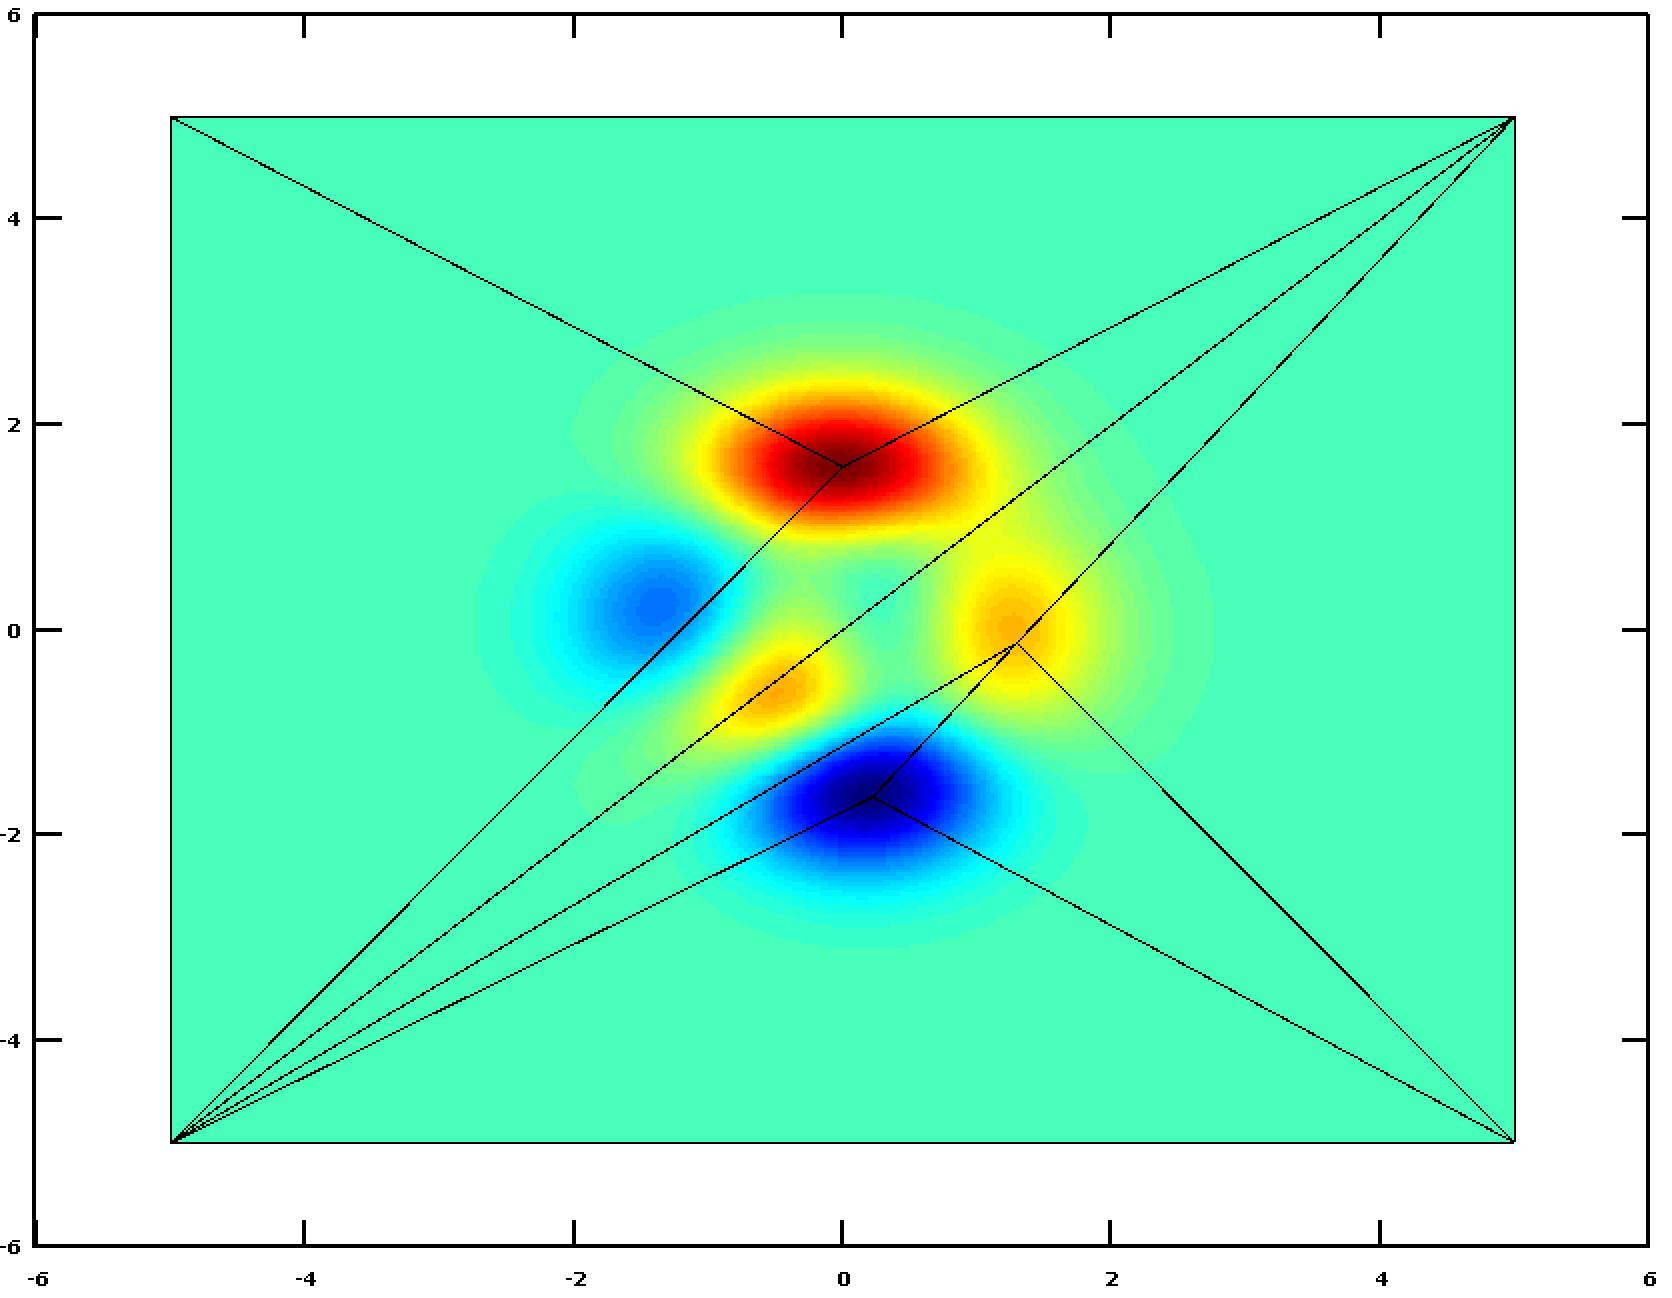
\includegraphics[width=50mm]{Figures/RefineOnly05.png}}
  \subfloat[$tol_{RD}=0.25$]{\label{fig_RefineOnlyB}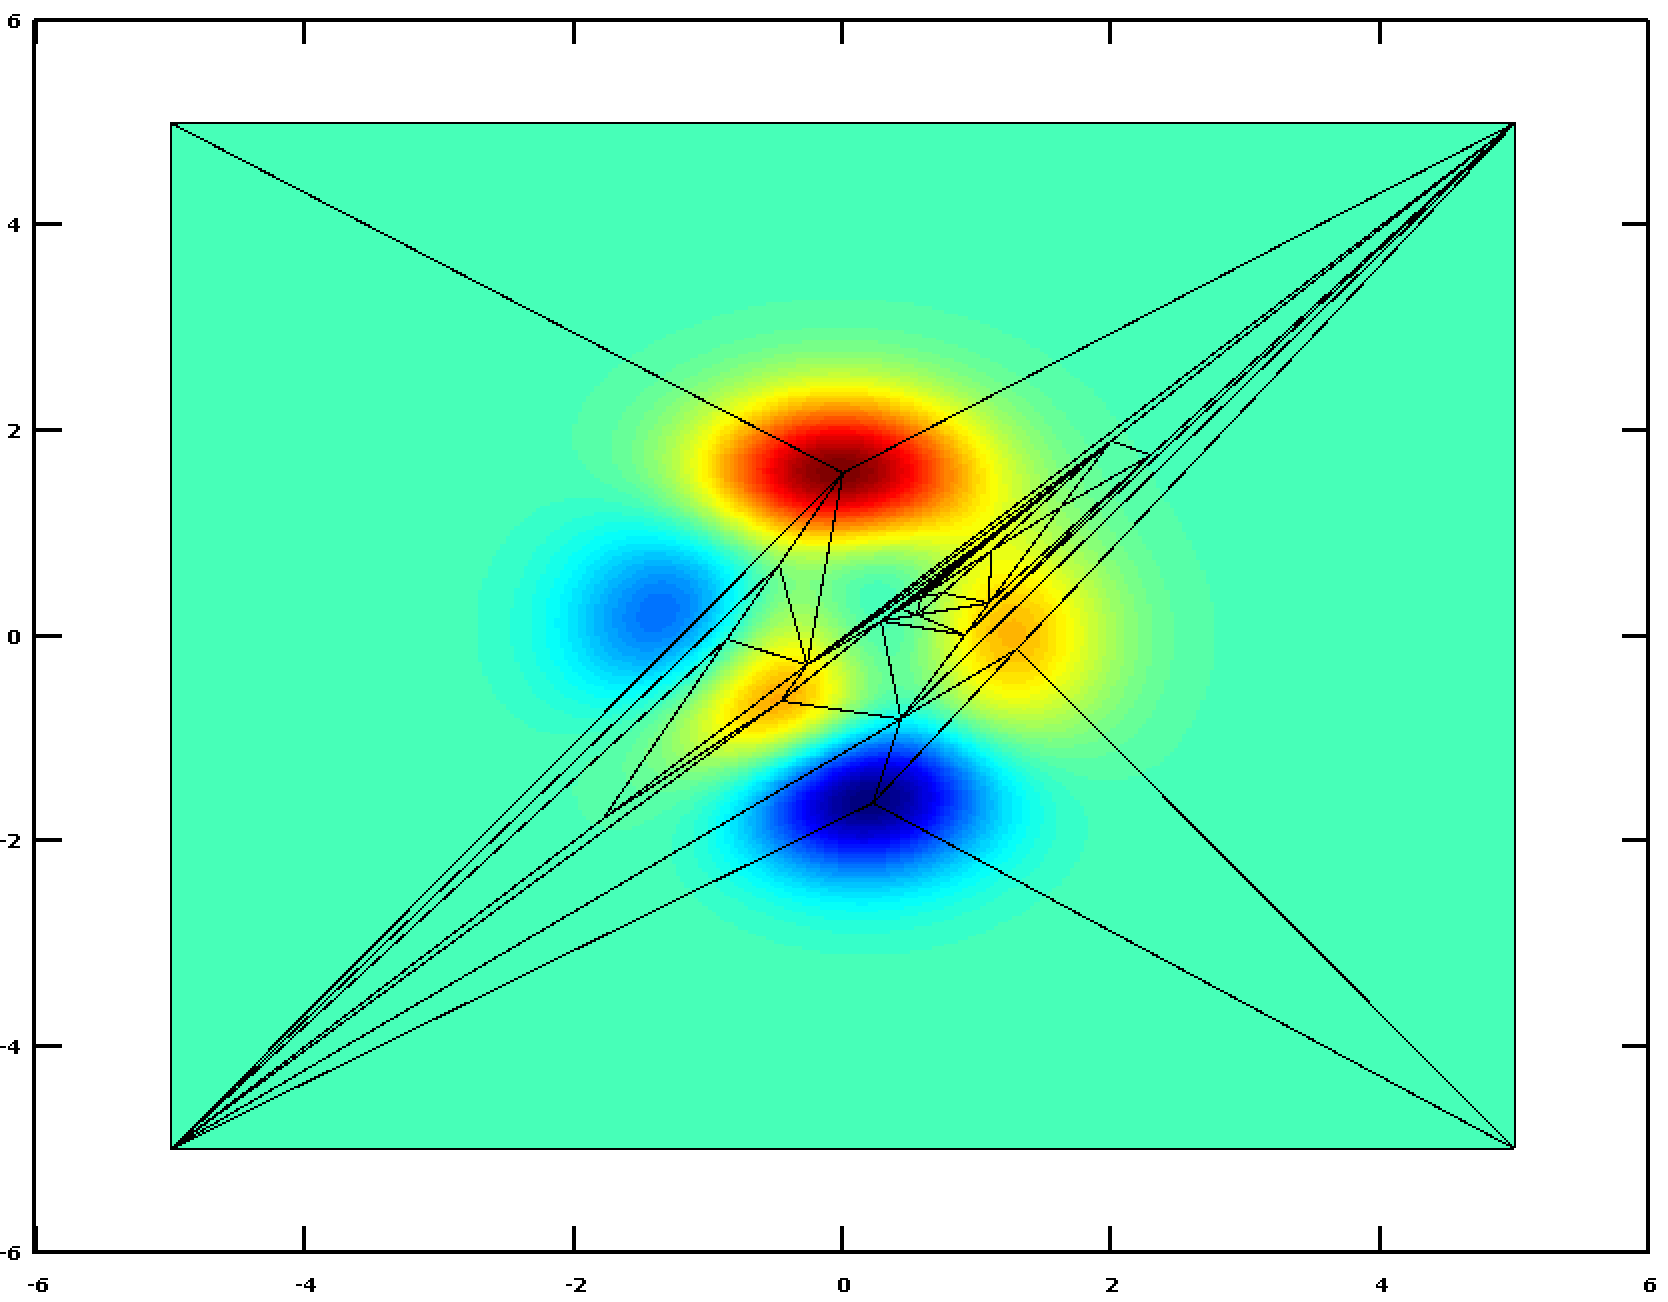
\includegraphics[width=50mm]{Figures/RefineOnly025.png}}
  \subfloat[$tol_{RD}=0.125$]{\label{fig_RefineOnlyC}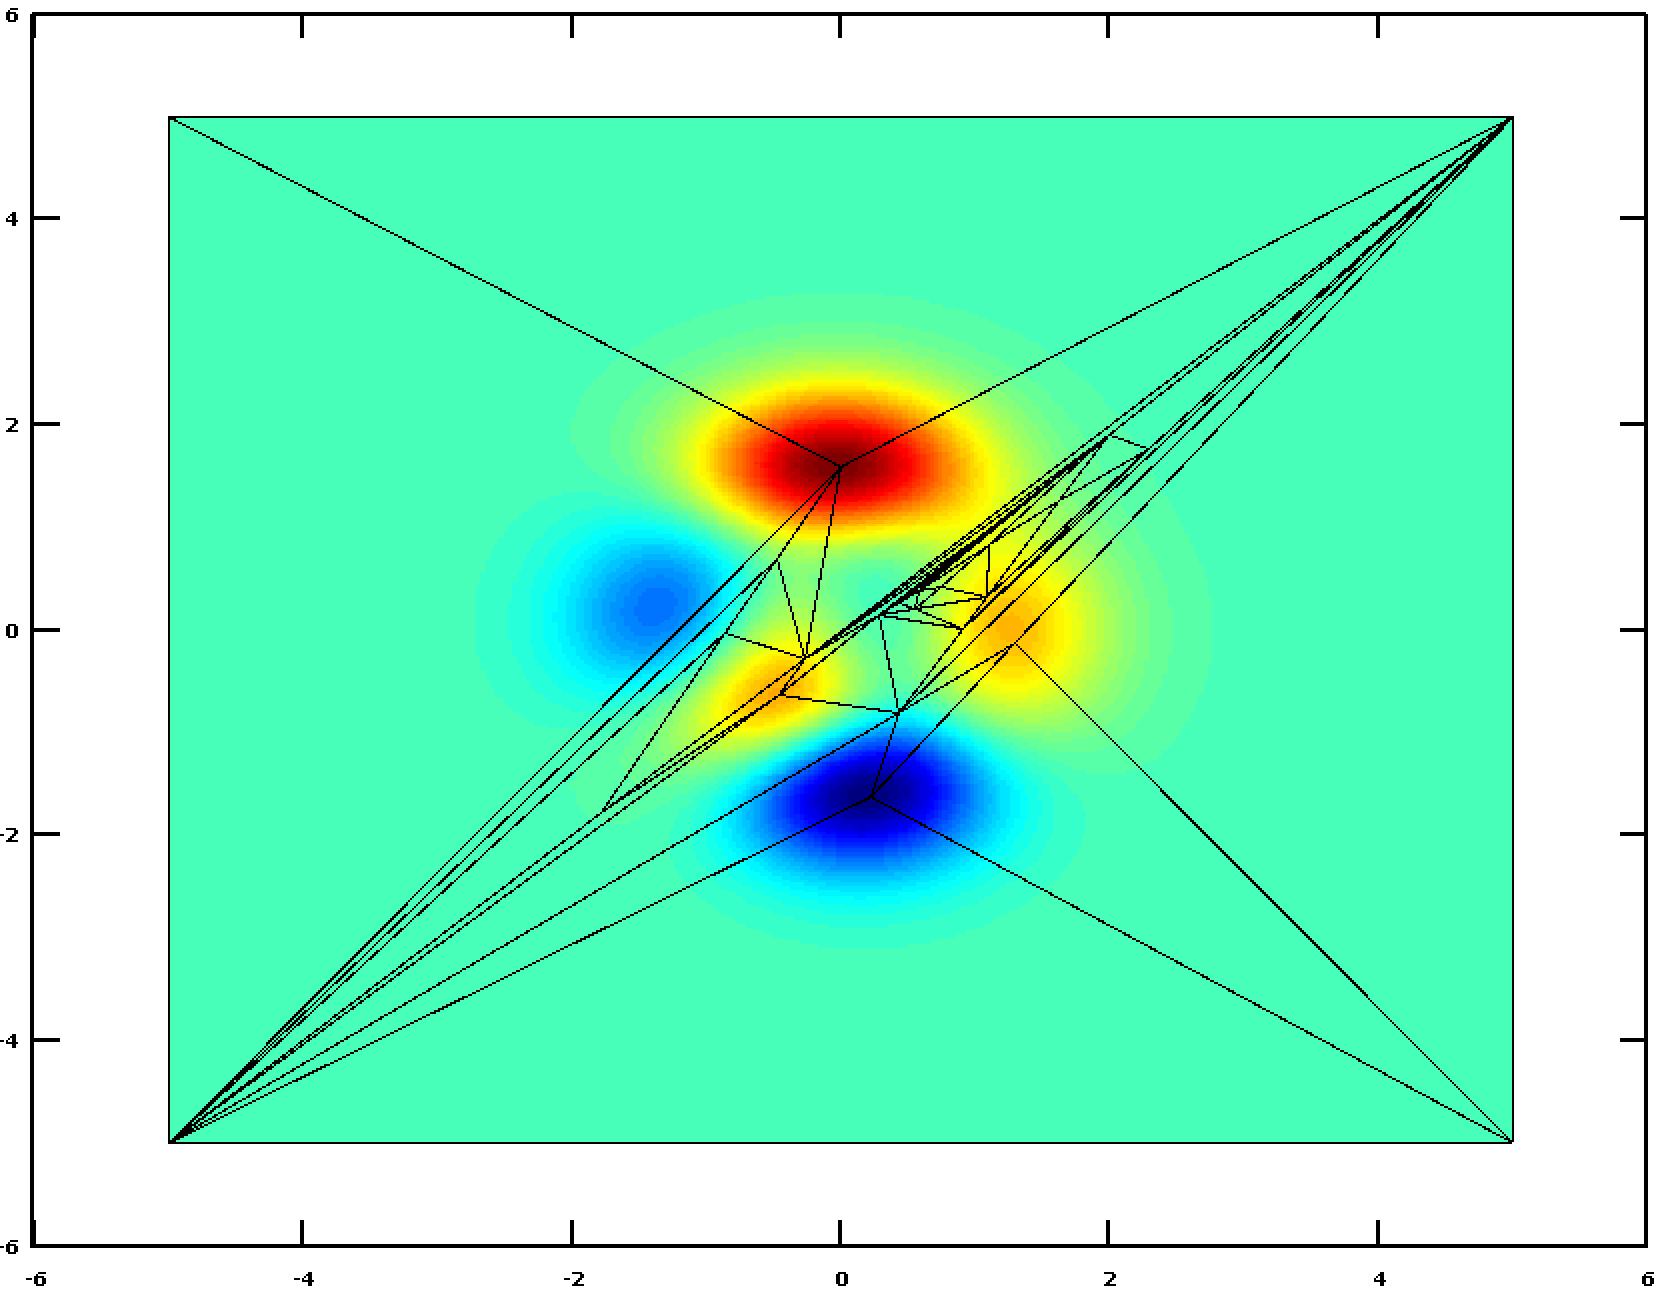
\includegraphics[width=50mm]{Figures/RefineOnly0125.png}}

  \caption{Mesh Refinement Only}
  \label{fig_RefineOnly}
  \end{center}
\end{figure}

In Fig. \ref{fig_RefineOnlyA}, it can be seen that only three nodes were
inserted. This is due to the very high value of $tol_{RD}$ for this
example.  However, nodes were inserted very near
to the local minima/maxima of the function. If $tol_{RD}$ were halved to
$0.25$, Fig. \ref{fig_RefineOnlyB} then $92$ nodes are inserted. Again, 
the
nodes are inserted very near to local minima/maxima and additionally
near saddle points. If $tol_{RD}$ is halved again to $0.125$,
Fig. \ref{fig_RefineOnlyC}, no more nodes are inserted. This is due to the
very poor quality triangles.  The sliver triangles that can be seen in
Fig. \ref{fig_RefineOnlyB} and Fig. \ref{fig_RefineOnlyC} represent a 
nearly planar 
section of the mesh and therefore is not refined further.  The 
major shortcoming of the developed algorithm is that element quality is 
not considered.  This limitation leads to poor quality meshes that 
cannot be refined further.

\subsection{Node Movement Effect}
In order to show the effect of node movement, the resultant mesh shown
in Fig. \ref{fig_RefineOnlyB} is used as input, and the same value for
$tol_{RD} = 0.25$ is used with Fig. \ref{alg_NodeSmoothing}.

\begin{figure}[h!]
  \begin{center}
 
  \subfloat[$tol_{RD}=0.25$]{\label{fig_NodeSmoothingA}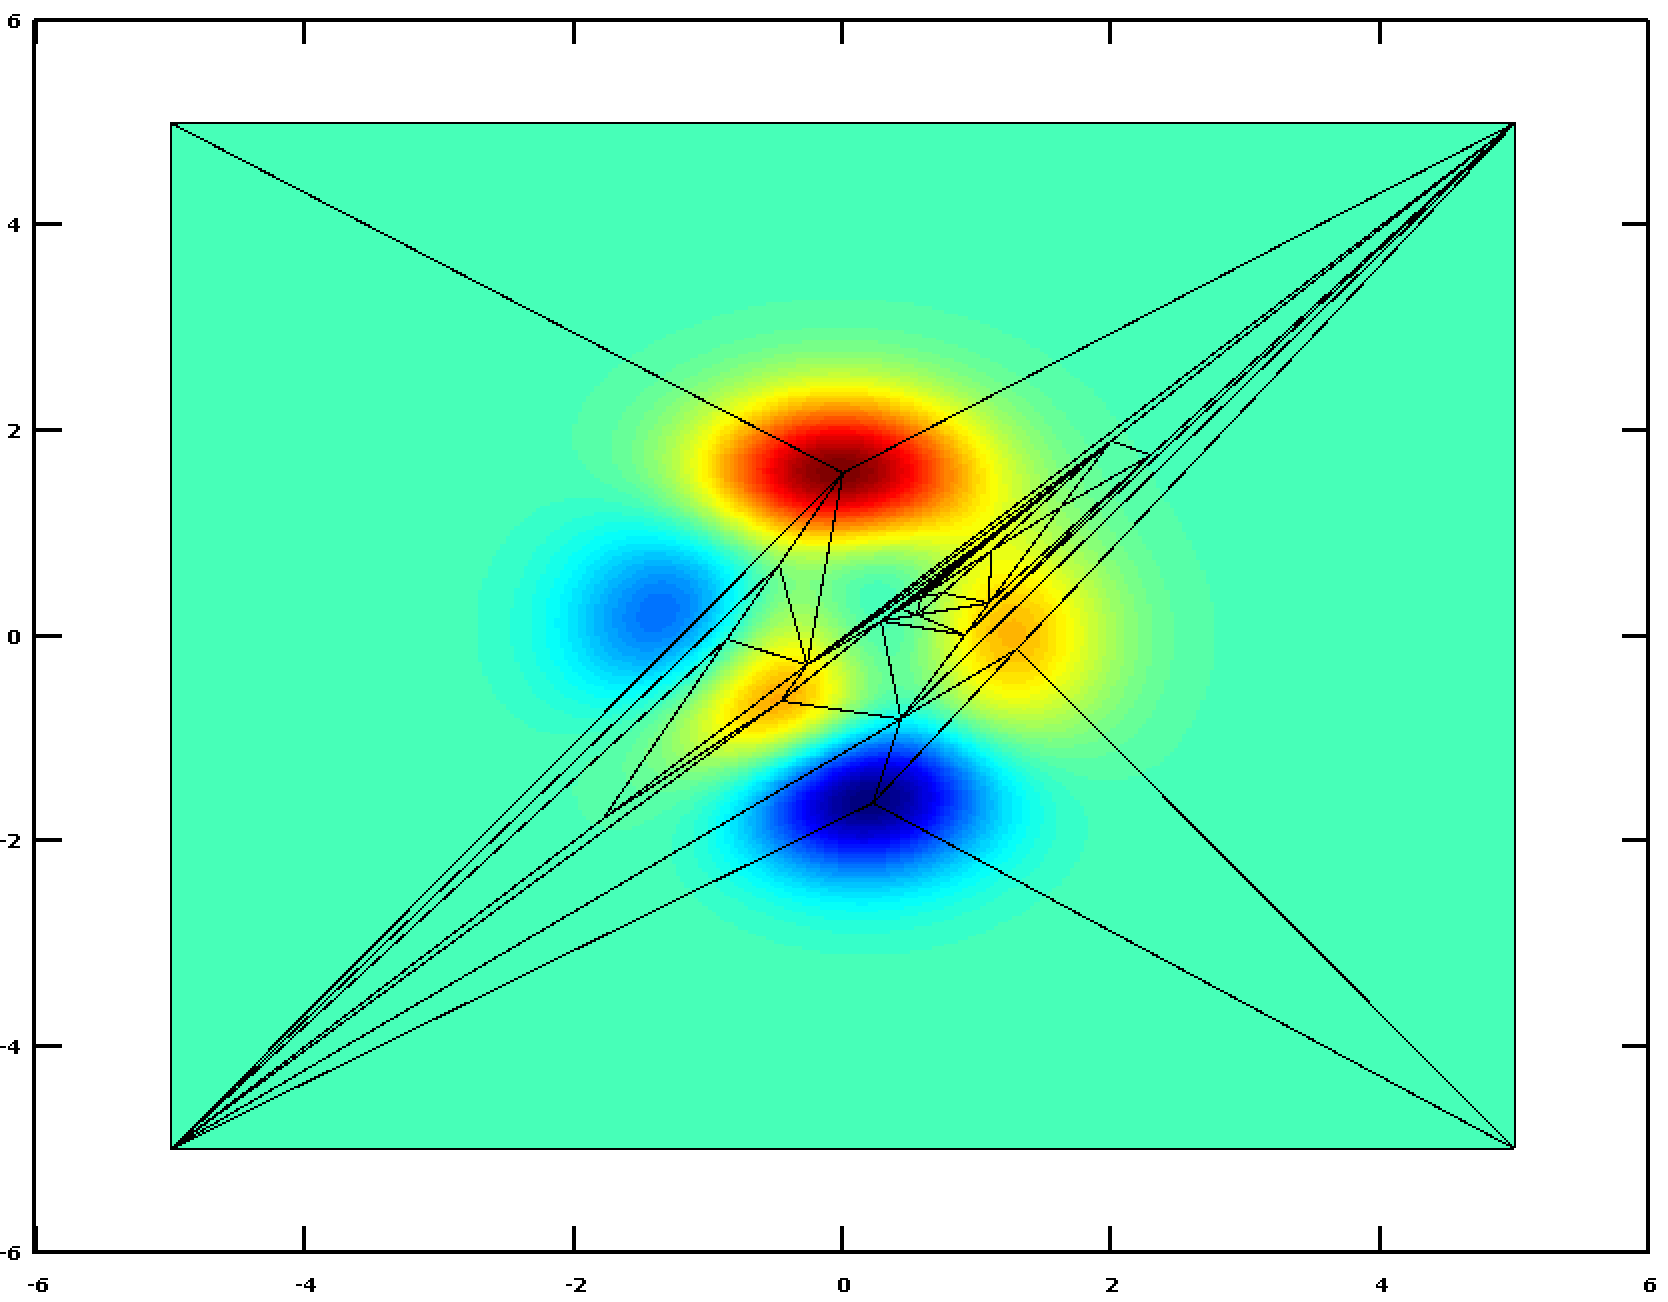
\includegraphics[width=60mm]{Figures/RefineOnly025.png}}
  \subfloat[$tol_{RD}=0.25$]{\label{fig_NodeSmoothingB}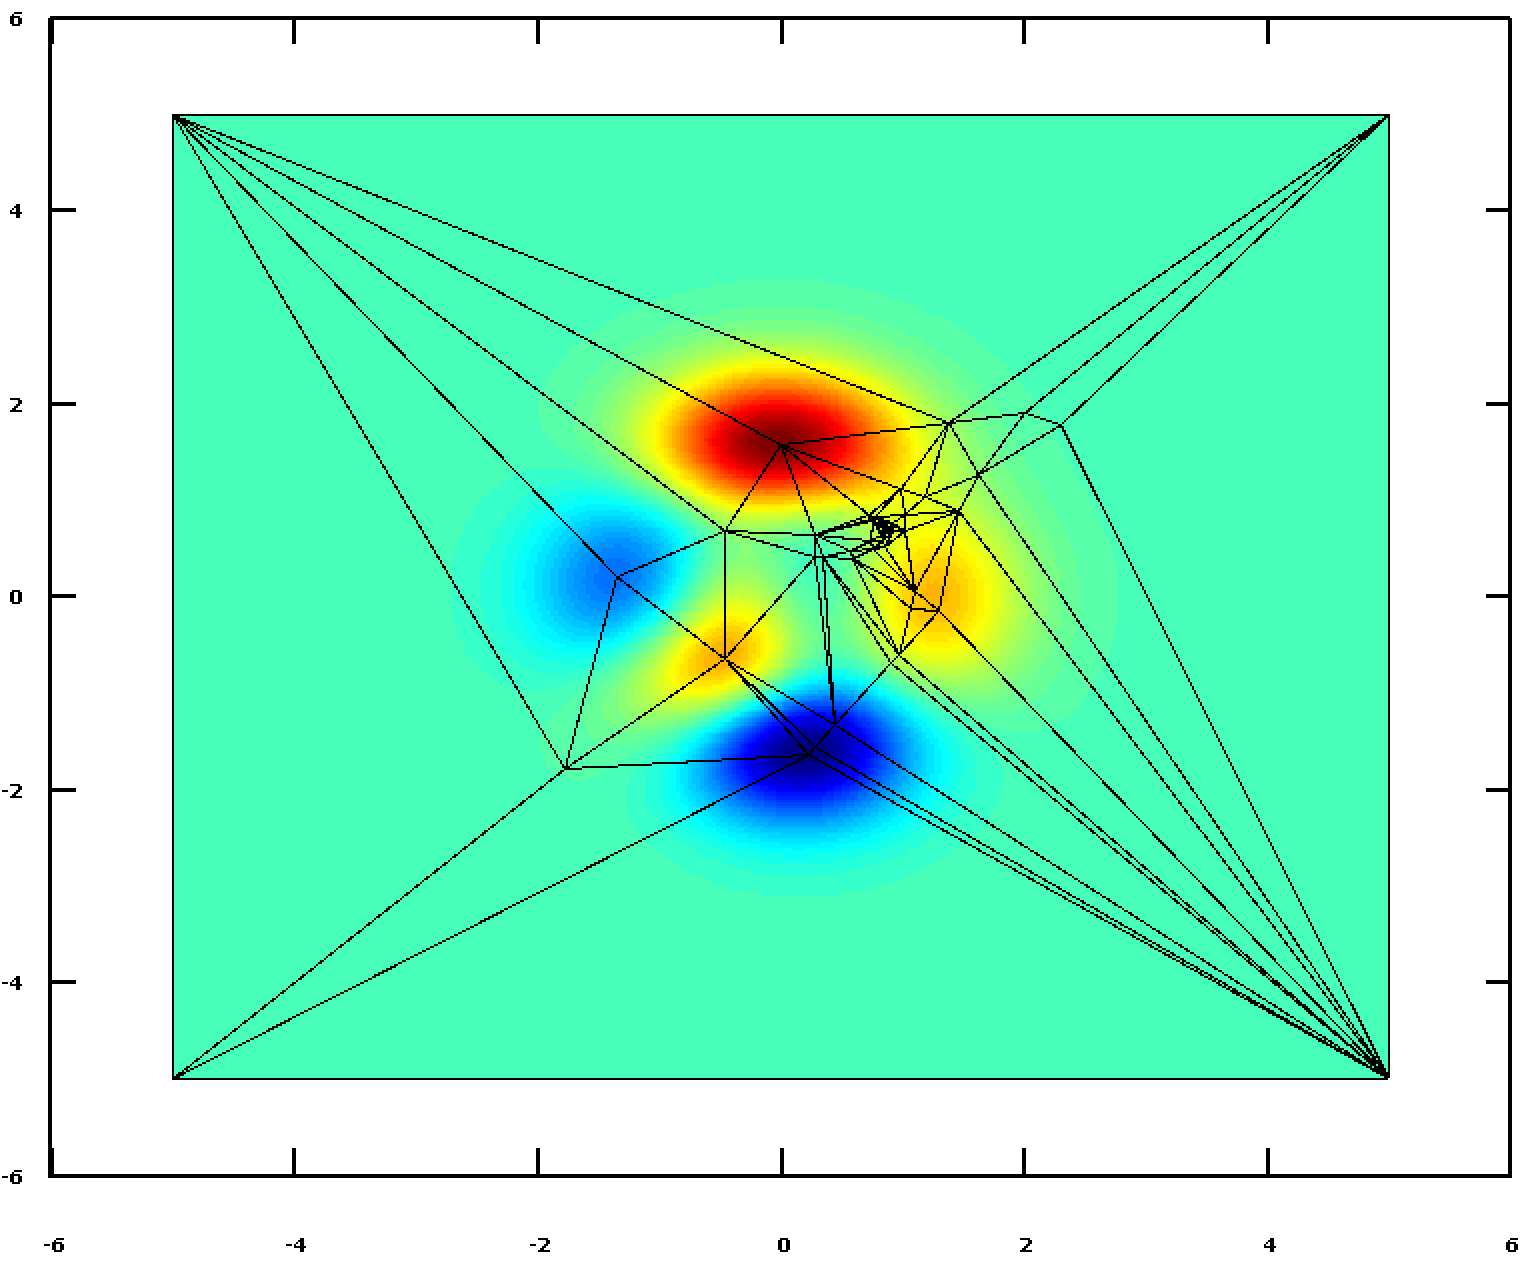
\includegraphics[width=60mm]{Figures/NodeSmooth025.png}}
  \caption{Effect of Node Movement on RD and Mesh Quality}
  \label{fig_NodeSmoothing}

  \end{center}
\end{figure}

Node movement was very effective at reducing representation deficit.
For this particular case, it reduced the representation deficit of the
input mesh by $23.36\%$. It should also be noted that the local
minima/maxima were accurately maintained by this procedure. It can also
be seen that moved nodes that were nearby but not in local minima/maxim
were moved to the local minima/maxima. Additionally, since the node
movement was allowed to perform local reconnections where needed
(discussed above), the element quality was also improved as a
side-effect.

\subsection{Effective Combination}
It is easily noted that while the aforementioned mesh operations are
effective at reducing representation deficit, they do not create high
quality triangles.  However, with the addition of a Delaunay local
reconnection pass in between refinement and node movement passes, the
element quality and representation deficit can be improved
significantly.

\begin{figure}[h!]
  \begin{center}
  \subfloat[$tol_{RD}=0.25$, no movement]{\label{fig_ComboA}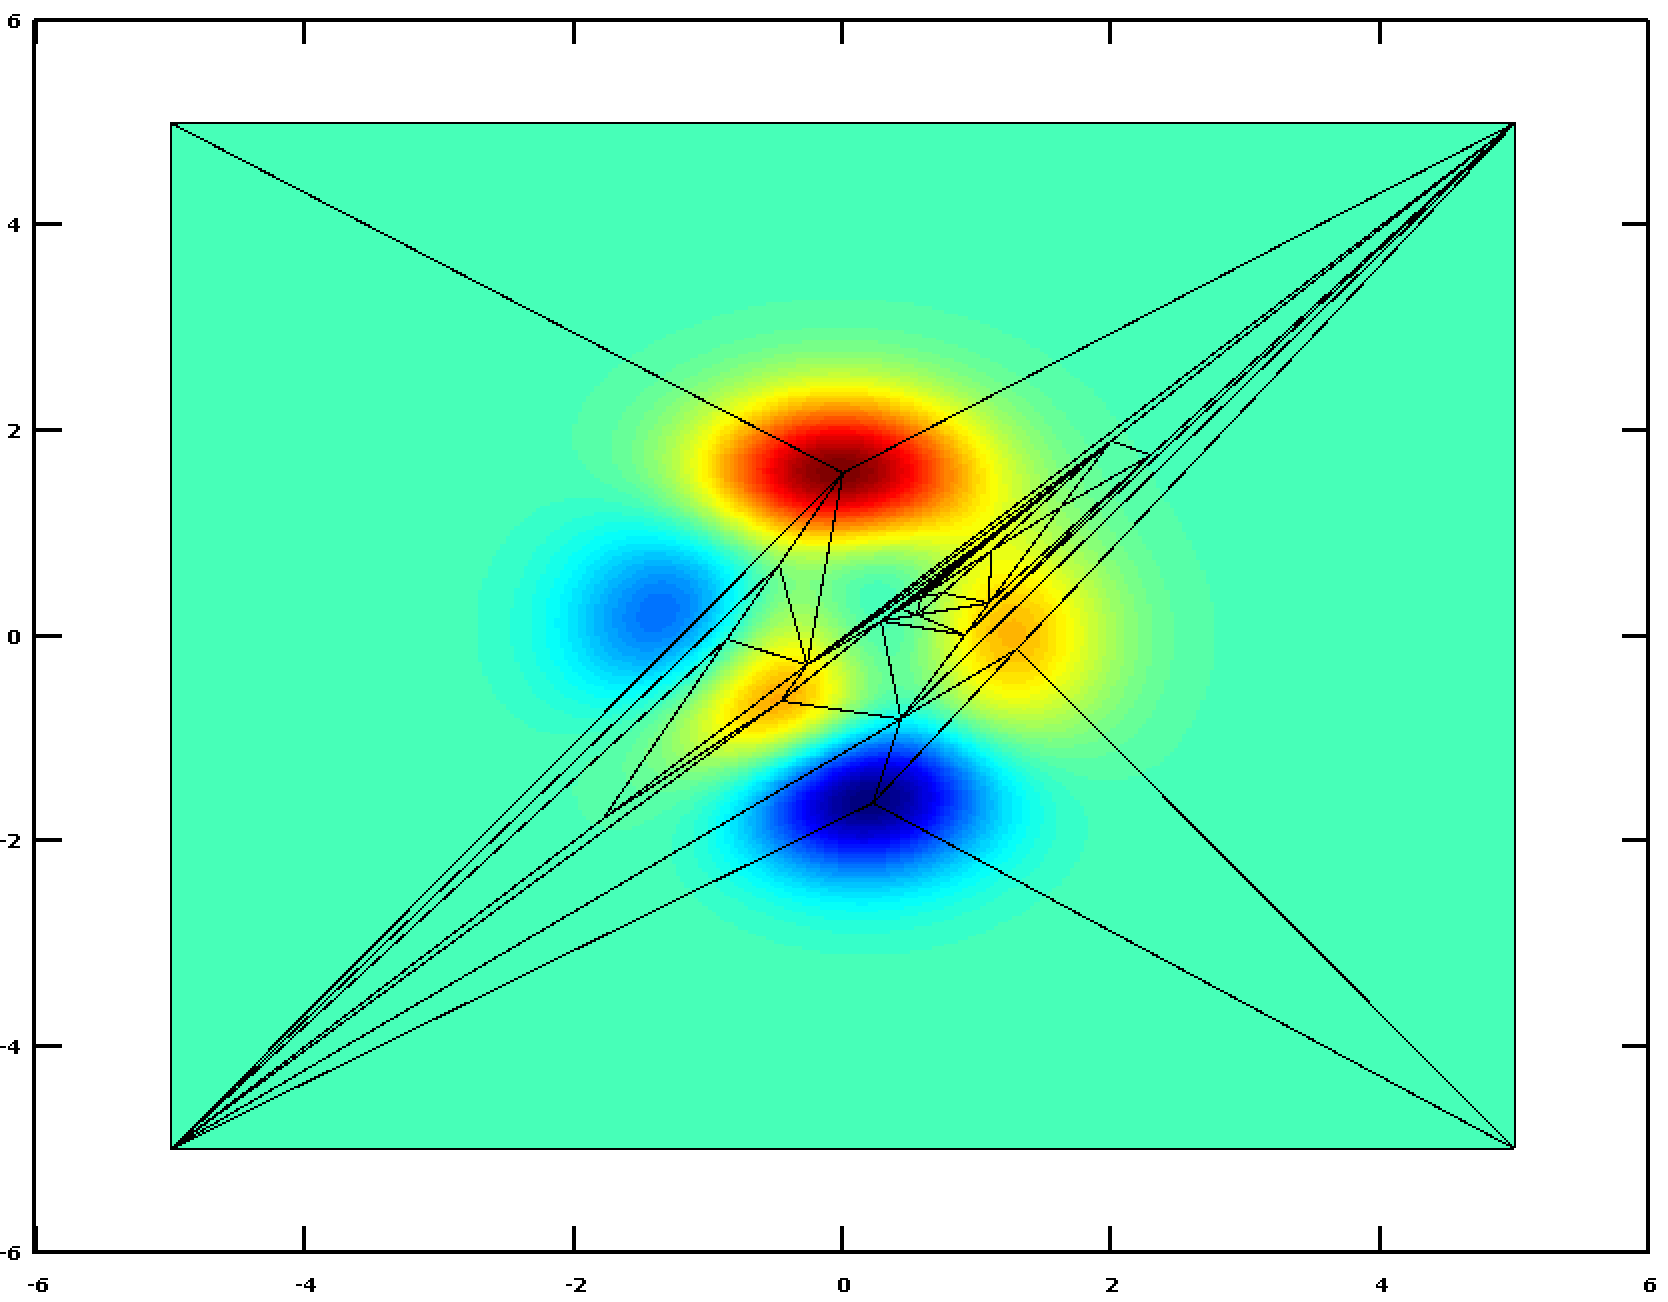
\includegraphics[width=50mm]{Figures/RefineOnly025.png}}
  \subfloat[$tol_{RD}=0.25$, movement post]{\label{fig_ComboB}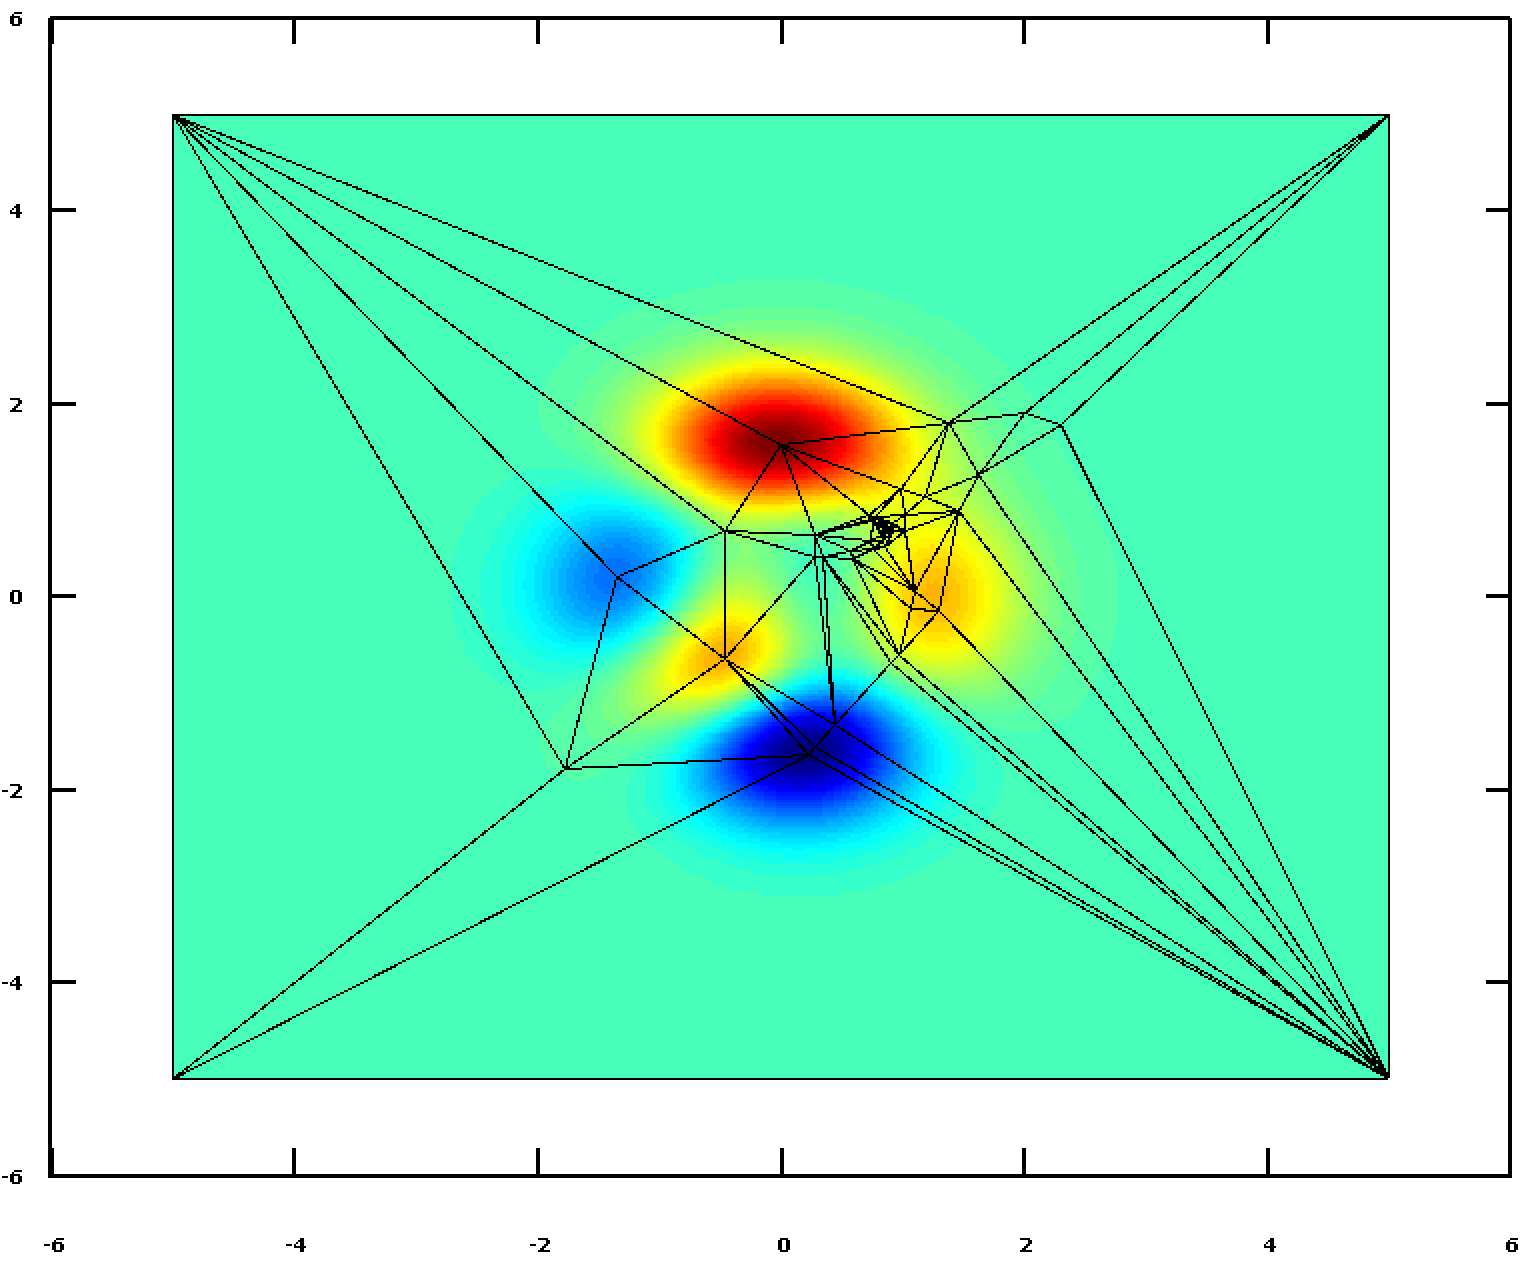
\includegraphics[width=50mm]{Figures/NodeSmooth025.png}}
  \subfloat[$tol_{RD}=0.25$, reconnection]{\label{fig_ComboC}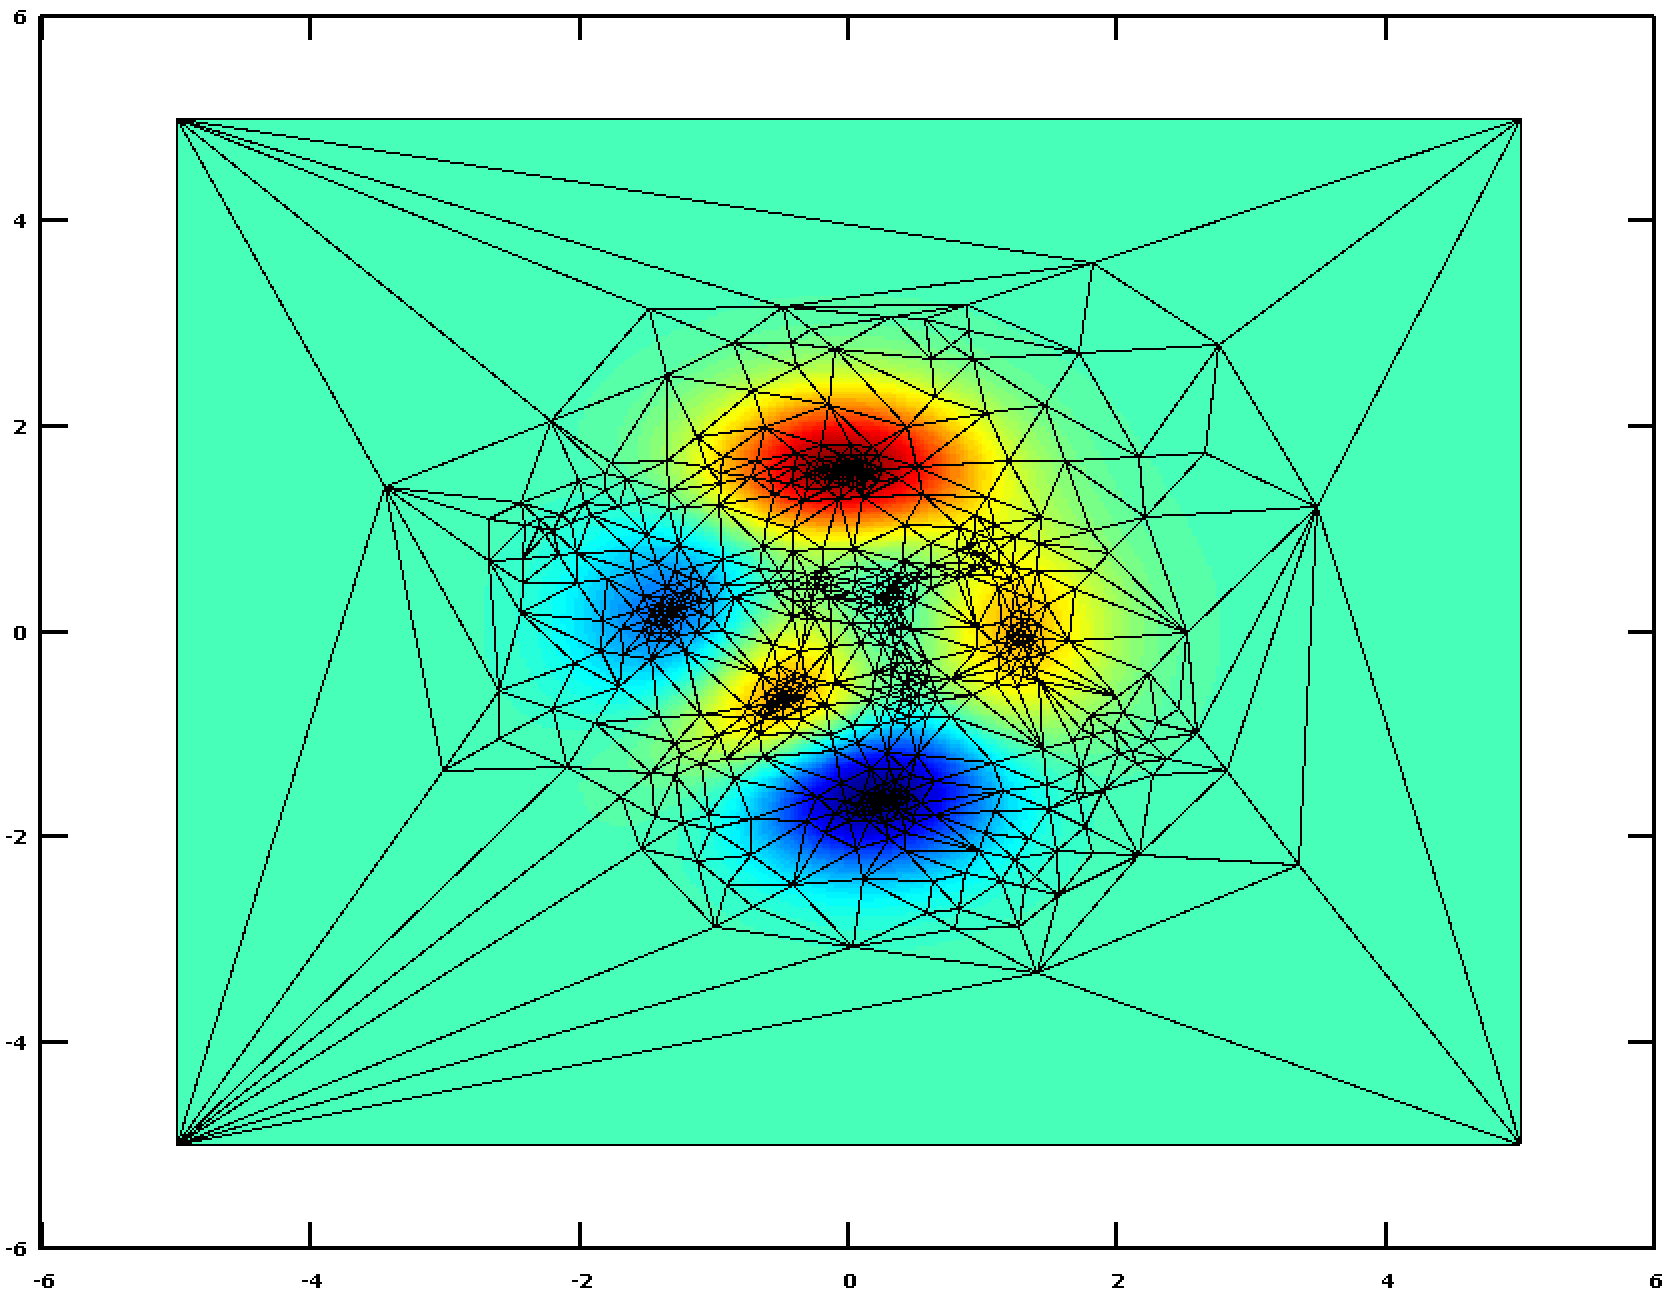
\includegraphics[width=50mm]{Figures/Reconnect025.png}}
  \caption{Comparison of Exclusive Splitting, with addition of Node
Movement, with further addition of local reconnection}
  \label{fig_NodeSmoothing}
  \end{center}
\end{figure}

[FIGURE ON MESH QUALITY]

In Fig. \ref{fig_ComboC}, the marked difference in mesh quality and mesh
density caused by local reconnection can be seen.  The addition of the
local reconnection enabled the triangle quality to be improved every
step and therefore allowed more nodes to be inserted. In this case, 
instead of $92$ nodes being inserted (Fig. \ref{fig_ComboA}), $713$ nodes 
were
inserted. The surface area of the final mesh was $179.234$. This is a
representation deficit of $0.725\%$.
[PARAGRAPH ON MESH QUALITY]

\begin{figure}[h!]
  \begin{center}
  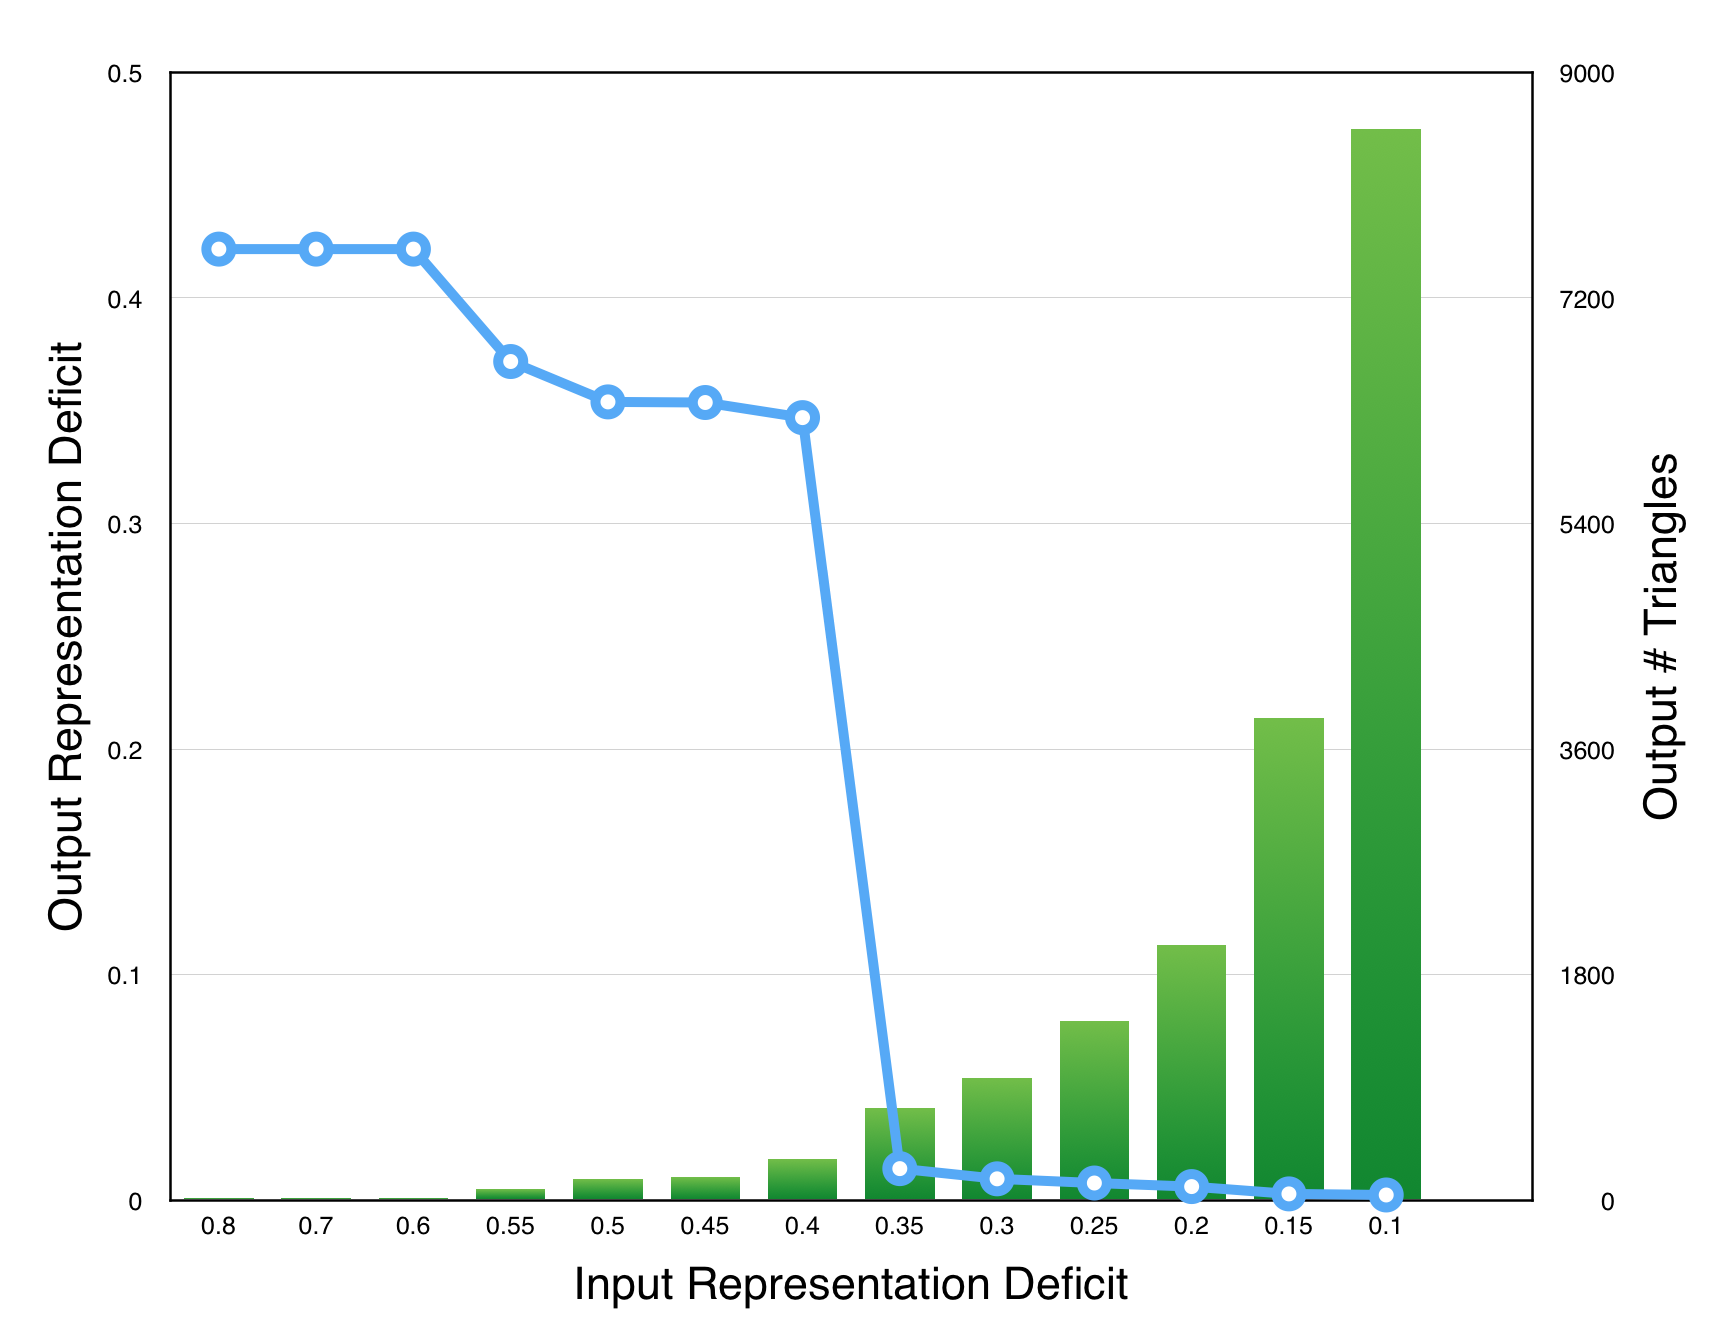
\includegraphics[width=90mm]{Figures/RDvsMeshSize.png}
  \caption{Output Surface $RD$ and Mesh Size vs. $tol_{RD}$}
  \label{fig_RDvsMeshSize}
  \end{center}
\end{figure}

A clear trend {\bf{Dave: A trend in what?}} can be seen in 
Fig. \ref{fig_RDvsMeshSize}; as the value of
$tol_{RD}$ is decreased, the representation deficit of the generated mesh
also decreases (blue line). Also, as with many optimization problems,
this particular geomtery (i.e., the ``peaks'' surface) and this particular 
initial mesh (i.e., which contains two triangles) have noticeable local 
minima in the search space.
Figure \ref{fig_RDvsMeshSize} clearly shows three plateaus of output
RD in the output mesh with decreasing $tol_{RD}$.  These occur at
$\sim42\%, \sim35\%,$ and $\sim1\%$.  The green bars depict the output
mesh size and also convey the diminishing returns of decreasing
$tol_{RD}$ too much. Only $18$ triangles are needed for the output RD to
reach $0.42$ ($42\%$).  However, an additional $156$ triangles were
needed to reduce the output RD by ten points ($\sim 35\%$). {\bf{Dave - 
I'm lost. What do you mean by 10 points?  10 percent?  10 fewer points 
(meaning nodes) in the mesh?}}  To get much closer to another local 
minimum (possibly the global minimum) many
more triangles were required, i.e., $738$ in total to reach $\sim 1\%$ 
output RD. In each case, the optimal substructure of the problem is 
apparent with the value of $tol_{RD}$ being greater than the 
representation deficit of the generated mesh.
